\section{外层求解}
\label{sec:bilevel-outer}

有了超梯度，外层就可以用前面各章的方法：$\bm{C}$是简单集合时用投影梯度（第~\ref{chap:feasible-iterations}章），变量多而问题光滑时用拟牛顿法（第~\ref{chap:quasi-newton}章），$\Phi$有折点时用非光滑方法（第~\ref{chap:nonsmooth-composite-optimization}章）。选择之前先要确定优化的是哪个目标：真实选解的$\Phi$，还是有限步的$\Phi_T$。

超梯度带着偏差时，外层能保证什么？若把带固定偏差的超梯度当成精确梯度，收敛结论就不成立了。下面按内层、导数、外层的顺序逐级核算。

\subsection{内层误差}
\label{sec:bilevel-inner-error}

内层算法停下时，手里是一个近似解$\hat{\bm{y}}$。这个点离内解有多远，可以用三个量来描述，它们含义不同，需要的计算条件也不同。

\paragraph{三种度量}
固定$\bm{x}$，记所选内解为$\bm{y}^\star$，定义
\[
 \delta=g(\bm{x},\hat{\bm{y}})-g(\bm{x},\bm{y}^\star),\qquad r=\lVert\nabla_{\bm{y}}g(\bm{x},\hat{\bm{y}})\rVert_2,\qquad d=\lVert\hat{\bm{y}}-\bm{y}^\star\rVert_2.
\]

$\delta$是内层目标差距，要知道最优值才能算。$r$是驻点残差，随手可算。$d$是到所选解的距离，通常没法直接算，而超梯度的误差恰恰取决于它。三者只有在特定条件下才能互相控制。

\begin{lemma}[强凸下的互控]
\label{lem:bilevel-inner-measures}
设对固定的$\bm{x}$，$\mu\bm{I}\preceq\nabla^2_{\bm{y}\bm{y}}g\preceq L_g\bm{I}$处处成立。则
\begin{align}
 \mu d&\leq r\leq L_gd,
 \label{eq:bilevel-inner-r}\\
 \frac{\mu}{2}d^2&\leq\delta\leq\frac{L_g}{2}d^2,
 \label{eq:bilevel-inner-delta}\\
 \frac{r^2}{2L_g}&\leq\delta\leq\frac{r^2}{2\mu}.
 \label{eq:bilevel-inner-pl}
\end{align}
\end{lemma}

\begin{proof}
记$\phi=g(\bm{x},\cdot)$，$\bm{e}=\hat{\bm{y}}-\bm{y}^\star$。由$\nabla\phi(\bm{y}^\star)=\bm{0}$和积分形式的中值定理，
\[
 \nabla\phi(\hat{\bm{y}})=\bar{\bm{H}}\bm{e},
\]
其中$\bar{\bm{H}}$是Hessian沿线段的平均，特征值在$[\mu,L_g]$内，这给出式~\eqref{eq:bilevel-inner-r}。

由Taylor公式，
\[
 \delta=\frac12\bm{e}^{\top}\tilde{\bm{H}}\bm{e},
\]
$\tilde{\bm{H}}$的特征值同样在$[\mu,L_g]$内，这给出式~\eqref{eq:bilevel-inner-delta}。

由强凸性，
\[
 \phi(\bm{y}^\star)\geq\phi(\hat{\bm{y}})-rd+\frac{\mu}{2}d^2\geq\phi(\hat{\bm{y}})-\frac{r^2}{2\mu},
\]
第二步是对$d$取最小，这给出式~\eqref{eq:bilevel-inner-pl}的右半。对左半，从$\hat{\bm{y}}$走一步梯度下降$\hat{\bm{y}}-\nabla\phi(\hat{\bm{y}})/L_g$，由下降引理，函数值至少下降$r^2/(2L_g)$，而它不会低于$\phi(\bm{y}^\star)$。
\end{proof}

\paragraph{条件去掉会怎样}
图~\ref{fig:bilevel-inner-measures}对比了强凸的$g=y^2/2$和平坦的$g=y^4/4$。对后者，$r=d^3$，$\delta=d^4/4$。当$d=0.1$时，残差只有$10^{-3}$，目标差距只有$2.5\times10^{-5}$，看上去已经收敛得很好，到解的距离却还有$0.1$。

\begin{BookInlineFigure}
 \centering
 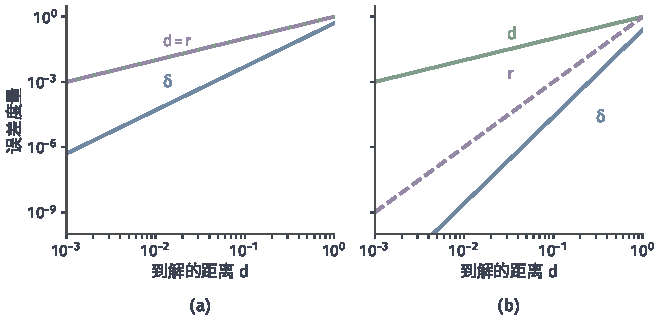
\includegraphics[width=112mm]{figures/05-optimization/07-multiple-criteria-and-nested-optimization/matplotlib/bilevel-inner-measures/figure.pdf}
 \caption{三种内层误差度量随距离$d$的变化，双对数坐标。(a)强凸的$g=y^2/2$：残差$r$（紫色虚线）与$d$（绿）重合，目标差距$\delta$（蓝）是$d^2/2$。(b)平坦的$g=y^4/4$：$r=d^3$，$\delta=d^4/4$，残差和目标差距都远小于到解的距离。}
 \label{fig:bilevel-inner-measures}
\end{BookInlineFigure}

非凸时情况更糟。$r=0$只说明是驻点，它可能是极大点或鞍点。即使是极小点，$d$也必须对着“所选解”算：$\delta$和$r$再小，也无法说明算法是否在正确的那个碗里。

\paragraph{热启动的得失}
外层变化不大时，内层从上一轮解继续，可以省去大量迭代，这是热启动的好处。第~\ref{sec:bilevel-switching}小节也展示了它的代价：它会一直追踪同一条局部分支，穿过切换点也不察觉。热启动减少重复求解，但不能免除全局选解的核对；内层非凸时，需要定期从不同初值重解内层，比较内层目标值。

\subsection{导数误差}
\label{sec:bilevel-derivative-error}

超梯度的误差有几个来源：内解没解准，所有二阶导数都算在错误的点上；伴随方程没解准；或者反传被截断。它们对外层方向的影响要分开看。

\paragraph{两项误差的分解}
记$\hat{\bm{H}}$、$\hat{\bm{B}}$是在$\hat{\bm{y}}$处计算的矩阵，$\bm{f}(\bm{y})=\nabla_{\bm{y}}F(\bm{x},\bm{y})$，并简写$\hat{\bm{f}}=\bm{f}(\hat{\bm{y}})$、$\bm{f}_\star=\bm{f}(\bm{y}^\star)$。设$\tilde{\bm{v}}$是伴随方程的近似解，残差和超梯度估计分别是
\begin{equation}
 \bm{r}_{\bm{v}}=\hat{\bm{H}}\tilde{\bm{v}}-\hat{\bm{f}},\qquad\hat{\bm{\gamma}}=\nabla_{\bm{x}}F(\bm{x},\hat{\bm{y}})-\hat{\bm{B}}^{\top}\tilde{\bm{v}}.
 \label{eq:bilevel-hypergradient-estimate}
\end{equation}

\begin{theorem}[超梯度误差的分解]
\label{thm:bilevel-hypergradient-error}
固定$\bm{x}$，设在$\bm{y}^\star$和$\hat{\bm{y}}$之间：$\bm{H}\succeq\mu\bm{I}$，$\lVert\hat{\bm{B}}\rVert_2\leq M_B$，$\lVert\bm{f}_\star\rVert_2\leq M_F$；$\nabla_{\bm{x}}F$、$\nabla_{\bm{y}}F$关于$\bm{y}$是$L_F$—Lipschitz的，$\bm{H}$、$\bm{B}$关于$\bm{y}$分别是$L_H$、$L_B$—Lipschitz的。记$d=\lVert\hat{\bm{y}}-\bm{y}^\star\rVert_2$。则
\begin{equation}
 \lVert\hat{\bm{\gamma}}-\nabla\Phi(\bm{x})\rVert_2\leq C_d\,d+\frac{M_B}{\mu}\lVert\bm{r}_{\bm{v}}\rVert_2,
 \label{eq:bilevel-hypergradient-error}
\end{equation}
其中常数为
\begin{equation}
 C_d=L_F+\frac{L_BM_F}{\mu}+\frac{M_B}{\mu}\Bigl(L_F+\frac{L_HM_F}{\mu}\Bigr).
 \label{eq:bilevel-hypergradient-constant}
\end{equation}
\end{theorem}

\begin{proof}
记$\bm{v}^\star=\bm{H}_\star^{-1}\bm{f}_\star$，由$\bm{H}_\star\succeq\mu\bm{I}$得$\lVert\bm{v}^\star\rVert_2\leq M_F/\mu$。在$\bm{B}$的差上加减一项，把误差拆成三部分：
\[
 \begin{aligned}
 \hat{\bm{\gamma}}-\nabla\Phi={}&\bigl[\nabla_{\bm{x}}F(\bm{x},\hat{\bm{y}})-\nabla_{\bm{x}}F(\bm{x},\bm{y}^\star)\bigr]\\
 &-(\hat{\bm{B}}-\bm{B}_\star)^{\top}\bm{v}^\star-\hat{\bm{B}}^{\top}(\tilde{\bm{v}}-\bm{v}^\star).
 \end{aligned}
\]

前两部分的范数分别不超过$L_Fd$和$L_BM_Fd/\mu$。第三部分要估计$\tilde{\bm{v}}-\bm{v}^\star$。由残差的定义和$\bm{f}_\star=\bm{H}_\star\bm{v}^\star$，得到
\[
 \hat{\bm{H}}(\tilde{\bm{v}}-\bm{v}^\star)=\bm{r}_{\bm{v}}+(\hat{\bm{f}}-\bm{f}_\star)-(\hat{\bm{H}}-\bm{H}_\star)\bm{v}^\star.
\]

两边乘$\hat{\bm{H}}^{-1}$并取范数，得到
\[
 \lVert\tilde{\bm{v}}-\bm{v}^\star\rVert_2\leq\frac{1}{\mu}\Bigl(\lVert\bm{r}_{\bm{v}}\rVert_2+L_Fd+\frac{L_HM_F}{\mu}d\Bigr).
\]
再乘$\lVert\hat{\bm{B}}\rVert_2\leq M_B$，三部分相加即得式~\eqref{eq:bilevel-hypergradient-error}。
\end{proof}

右端第一项由内层距离$d$负责，第二项由伴随残差负责，两者互不替代。只把$d$压小而不解准伴随方程，或者反过来，都会停在另一项决定的误差水平上。迭代展开时第二项换成式~\eqref{eq:bilevel-truncation}的截断误差。这些结论都要有相应的稳定性条件：$\mu$变小，所有系数都变大；$\bm{H}$奇异时上界不成立。

\paragraph{手算一次}
正则拟合例在$x=1$处，$y^\star=3/2$，$\Phi'(1)=-3/8$。设内层只解到$\hat{y}=1.4$，$d=0.1$，这时$\hat{H}=2$，$\hat{B}=1.4$，$\partial_yF=0.4$。伴随方程精确解是$\hat{v}=0.2$，超梯度估计和误差分别是
\[
 \hat{\gamma}=-0.28,\qquad\lvert\hat{\gamma}-\Phi'(1)\rvert=0.095.
\]

若再把伴随方程解错，取$\tilde{v}=0.15$，残差是$r_v=2\times0.15-0.4=-0.1$，则
\[
 \tilde{\gamma}=-0.21,\qquad\lvert\tilde{\gamma}-\Phi'(1)\rvert=0.165.
\]

代入式~\eqref{eq:bilevel-hypergradient-constant}。这里$L_F=L_B=1$，$L_H=0$，$\mu=2$，$M_F=1/2$，$M_B=1.4$，所以$C_d=1.95$，式~\eqref{eq:bilevel-hypergradient-error}的右端是
\[
 1.95\times0.1+0.7\times0.1=0.265.
\]
它确实是$0.165$的上界。

\paragraph{用数值实验看两项}
图~\ref{fig:bilevel-error-grid}用一个$d=30$的正则最小二乘内层，同时改变内层步数$K$和共轭梯度步数$k$。(a)中$k$固定时，增加$K$只能把误差压到某个平台，平台高度由$k$决定。(b)中$K$固定时，增加$k$也只能压到由$K$决定的平台。两个旋钮要一起拧，单独加大其中一个是浪费。

\begin{BookInlineFigure}
 \centering
 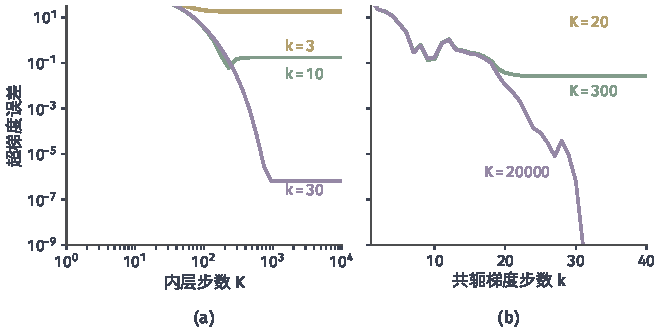
\includegraphics[width=112mm]{figures/05-optimization/07-multiple-criteria-and-nested-optimization/matplotlib/bilevel-error-grid/figure.pdf}
 \caption{超梯度误差的两个来源。内层是$d=30$的正则最小二乘，$x=0.05$，$\kappa\approx48$，数据由固定种子生成；内层用从零出发的梯度下降，步长$1/L_g$，伴随方程用共轭梯度法。(a)固定$k=3,10,30$，误差随内层步数$K$的变化。(b)固定$K=20,300,20000$，误差随共轭梯度步数$k$的变化。}
 \label{fig:bilevel-error-grid}
\end{BookInlineFigure}

\subsection{外层误差}
\label{sec:bilevel-outer-error}

最后把内层和导数的误差接到外层。本小节要解决的问题是：外层迭代用的是有偏差的超梯度，最终能保证什么，以及什么时候应该停下。

\paragraph{主要思想：偏差决定下限}
外层最简单的情形是无约束的梯度下降，用带误差$\bm{e}^{(t)}$的估计代替真实梯度：
\[
 \hat{\bm{\gamma}}^{(t)}=\nabla\Phi(\bm{x}^{(t)})+\bm{e}^{(t)}.
\]
下面的定理说明，偏差会直接进入驻定精度。

\begin{theorem}[带误差的外层梯度下降]
\label{thm:bilevel-inexact-outer}
设$\Phi$有下界$\Phi_{\inf}$，梯度在含迭代点的区域上$L_{\Phi}$—Lipschitz。迭代
\begin{equation}
 \bm{x}^{(t+1)}=\bm{x}^{(t)}-\frac{1}{L_{\Phi}}\hat{\bm{\gamma}}^{(t)}
 \label{eq:bilevel-outer-update}
\end{equation}
满足
\begin{equation}
 \min_{0\leq t<T}\lVert\nabla\Phi(\bm{x}^{(t)})\rVert_2^2\leq\frac{2L_{\Phi}\bigl(\Phi(\bm{x}^{(0)})-\Phi_{\inf}\bigr)}{T}+\frac1T\sum_{t=0}^{T-1}\lVert\bm{e}^{(t)}\rVert_2^2.
 \label{eq:bilevel-inexact-outer}
\end{equation}
\end{theorem}

\begin{proof}
记$\bm{\gamma}=\nabla\Phi(\bm{x}^{(t)})$，$\hat{\bm{\gamma}}=\bm{\gamma}+\bm{e}$，略去上标。由下降引理，
\[
 \Phi(\bm{x}^{(t+1)})\leq\Phi(\bm{x}^{(t)})-\frac{1}{L_{\Phi}}\langle\bm{\gamma},\hat{\bm{\gamma}}\rangle+\frac{1}{2L_{\Phi}}\lVert\hat{\bm{\gamma}}\rVert_2^2.
\]

利用恒等式
\[
 2\langle\bm{\gamma},\hat{\bm{\gamma}}\rangle=\lVert\bm{\gamma}\rVert_2^2+\lVert\hat{\bm{\gamma}}\rVert_2^2-\lVert\bm{e}\rVert_2^2,
\]
$\lVert\hat{\bm{\gamma}}\rVert_2^2$项正好抵消，得到
\[
 \Phi(\bm{x}^{(t+1)})\leq\Phi(\bm{x}^{(t)})-\frac{1}{2L_{\Phi}}\lVert\bm{\gamma}\rVert_2^2+\frac{1}{2L_{\Phi}}\lVert\bm{e}\rVert_2^2.
\]

对$t$从$0$到$T-1$求和，用$\Phi(\bm{x}^{(T)})\geq\Phi_{\inf}$，两边乘$2L_{\Phi}/T$，再用最小值不超过平均值即得。
\end{proof}

若偏差始终约为$\varepsilon$，式~\eqref{eq:bilevel-inexact-outer}右端第二项约为$\varepsilon^2$，不随$T$减小，这个上界只能保证$\lVert\nabla\Phi\rVert_2$降到$\varepsilon$的量级。要得到收敛，内层精度必须随外层进展提高，比如让$\sum_t\lVert\bm{e}^{(t)}\rVert_2^2$有限，这时第二项按$1/T$衰减。

这正对应图~\ref{fig:bilevel-outer-bias}。正则拟合例取$\eta=1$，从$x^{(0)}=1$出发，内层跑固定的$K$步后代入隐式公式。$K=2$时迭代收敛到$x=5/3$，这里$\hat{y}=1$，估计的超梯度为零，真实梯度却是$-27/512$。$K$增大时偏差缩小但不消失，只有$K$随$t$增长时才收敛到$x=2$。

\begin{BookInlineFigure}
 \centering
 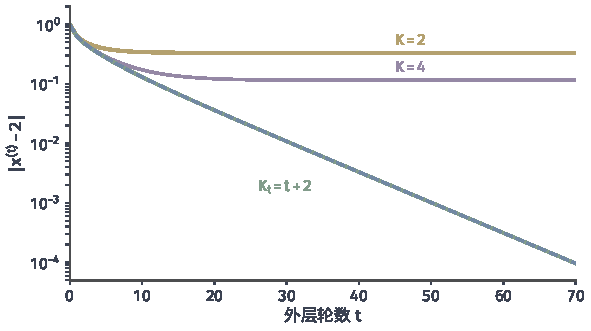
\includegraphics[width=100mm]{figures/05-optimization/07-multiple-criteria-and-nested-optimization/matplotlib/bilevel-outer-bias/figure.pdf}
 \caption{外层迭代误差$\lvert x^{(t)}-2\rvert$，正则拟合例，外层步长$\eta=1$，$x^{(0)}=1$，内层每轮从$y^{(0)}=0$跑$K$步后用隐式公式。黄线$K=2$、紫线$K=4$停在偏差决定的平台，绿线$K_t=t+2$与精确内解（蓝色虚线）几乎重合，持续收敛。}
 \label{fig:bilevel-outer-bias}
\end{BookInlineFigure}

\paragraph{计算过程}
把整个外层循环在这个例子上走几轮，内层步数取$K_t=t+2$。

\needspace{6\baselineskip}
\paragraph{变量}
\begin{itemize}
 \item 外层迭代点$x^{(t)}$，外层步长$\eta$。
 \item 内层输出$\hat{y}$，内层残差$r=(1+x)\hat{y}-3$。
 \item 伴随解$v$，超梯度估计$\hat{\gamma}$。
\end{itemize}

\paragraph{初始化}
例中$x^{(0)}=1$，$\eta=1$。正则拟合例在$x\geq1$上$\lvert\Phi''\rvert\leq15/16$，步长$\eta=1$略小于$1/L_{\Phi}=16/15$，定理~\ref{thm:bilevel-inexact-outer}的证明同样适用，只需把$L_{\Phi}$换成$1/\eta$。

\needspace{6\baselineskip}
\paragraph{每轮更新}
\begin{enumerate}
 \item 内层从$y^{(0)}=0$运行$K_t$步，由式~\eqref{eq:bilevel-ridge-finite}得到$\hat{y}$，并记录残差$r$。

 例中第一轮$x=1$，$q=0$，$\hat{y}=3/2$，残差为$0$。

 \item 解伴随方程，由式~\eqref{eq:bilevel-hypergradient-estimate}得到超梯度估计。

 例中$H=1+x$，$\partial_yF=\hat{y}-1$，$B=\hat{y}$，第一轮的结果是
 \[
  v=\frac{\hat{y}-1}{1+x}=\frac14,\qquad\hat{\gamma}=-\hat{y}v=-\frac38.
 \]

 \item 更新外层变量：$x^{(t+1)}=x^{(t)}-\eta\hat{\gamma}$。

 例中第一轮得到$x^{(1)}=11/8=1.375$。后面几轮的数值见表~\ref{tab:bilevel-outer-rounds}。
\end{enumerate}

\begin{BookInlineTable}
 \centering
 \begin{tabular}{rrrrrrr}
  \toprule
  $t$ & $K_t$ & $x^{(t)}$ & $\hat{y}$ & $r$ & $\hat{\gamma}$ & $\Phi'$\\
  \midrule
  $0$ & $2$ & $1.0000$ & $1.5000$ & $0.0000$ & $-0.3750$ & $-0.3750$\\
  $1$ & $3$ & $1.3750$ & $1.2715$ & $0.0198$ & $-0.1453$ & $-0.1400$\\
  $2$ & $4$ & $1.5203$ & $1.1849$ & $-0.0137$ & $-0.0869$ & $-0.0899$\\
  $3$ & $5$ & $1.6072$ & $1.1536$ & $0.0077$ & $-0.0680$ & $-0.0665$\\
  $4$ & $6$ & $1.6752$ & $1.1197$ & $-0.0044$ & $-0.0501$ & $-0.0509$\\
  \bottomrule
 \end{tabular}
 \caption{正则拟合例的外层循环，$\eta=1$，内层步数$K_t=t+2$。最后一列是在当前$x^{(t)}$处的真实超梯度。}
 \label{tab:bilevel-outer-rounds}
\end{BookInlineTable}

最终$x^{(t)}$趋于$x=2$。表中$\hat{\gamma}$与真实导数的差随内层残差缩小，这就是定理~\ref{thm:bilevel-hypergradient-error}所说的情况。

\paragraph{报告什么、何时停止}
外层的停止不能只看损失曲线，下面四项要分别检查，其中任何一项不达标都不能得出结论。

\begin{itemize}
 \item 外层可行性：$\bm{x}\in\bm{C}$是否成立，$\bm{x}$是否在$\operatorname{dom}\bm{S}$内，也就是内层确实有解。
 \item 外层驻定：有约束时用投影梯度的残差，无约束时用$\lVert\hat{\bm{\gamma}}\rVert_2$，并以估计的偏差为基准；$\lVert\hat{\bm{\gamma}}\rVert_2$低于偏差水平时继续迭代已没有依据。
 \item 内层误差：驻点残差或目标差距；非凸时再比较不同初值下的内层目标值。
 \item 导数误差：伴随残差或截断长度，并可用$\Phi$的中心差分抽查几个方向，差分时内层要解得足够准。
\end{itemize}

\paragraph{成本核算}
总成本要把四个部分分开算。设外层跑$T_{\mathrm{o}}$轮，每轮内层$K$步、共轭梯度$k$步，内层梯度的成本记作一个单位，Hessian向量积是它的常数倍。隐式微分的总计算量约是$T_{\mathrm{o}}(K+ck)$个单位，$c$是这个常数倍数，存储是$O(d)$。反向展开的计算量约是$cT_{\mathrm{o}}K$，存储变成$O(Kd)$，用检查点可以再压缩。内层病态时$K$和$k$都要增大，这是这类方法最主要的成本。

\paragraph{局部结论与全局结论}
定理~\ref{thm:bilevel-inexact-outer}只保证驻定，而$\Phi$一般是非凸的。即使内层对$y$强凸、外层对$y$凸，$\Phi$也可能非凸：正则拟合例有
\[
 \Phi''(x)=\frac{27-6u}{u^4},\qquad u=1+x,
\]
在$x>7/2$时为负。内层非凸时问题更严重，第~\ref{sec:bilevel-switching}小节的例子中$\Phi$还会跳变。所以局部收敛的结果，加上驻定残差很小，都不能自动说成整个双层问题的全局最优。要作全局的声明，需要多初值搜索或问题本身的结构，并如实说明已检查的范围。
